%%% File-Information {{{
%%% Filename: template_bericht.tex
%%% Purpose: lab report, technical report, project report
%%% Time-stamp: <2004-06-22 23:36:32 xx>
%%% Authors: The LaTeX@TUG-Team [http://latex.tugraz.at/]:
%%%          Karl Voit (vk), Michael Prokop (mp), Stefan Sollerer (ss)
%%% History:
%%%   20040625 (vk,ss) initial version
%%%
%%% Notes:
%%%
%%%
%%%
%%% }}}
%%%%%%%%%%%%%%%%%%%%%%%%%%%%%%%%%%%%%%%%%%%%%%%%%%%%%%%%%%%%%%%%%%%%%%%%%%%%%%%%
%%% main document {{{

\documentclass[
a4paper,     %% defines the paper size: a4paper (default), a5paper, letterpaper, ...
% landscape,   %% sets the orientation to landscape
% twoside,     %% changes to a two-page-layout (alternatively: oneside)
% twocolumn,   %% changes to a two-column-layout
 headsepline, %% add a horizontal line below the column title
% footsepline, %% add a horizontal line above the page footer
% titlepage,   %% only the titlepage (using titlepage-environment) appears on the first page (alternatively: notitlepage)
 parskip=half,
% halfparskip,     %% insert an empty line between two paragraphs (alternatively: halfparskip, ...)
% leqno,       %% equation numbers left (instead of right)
 fleqn,       %% equation left-justified (instead of centered)
% tablecaptionabove, %% captions of tables are above the tables (alternatively: tablecaptionbelow)
% draft,       %% produce only a draft version (mark lines that need manual edition and don't show graphics)
% 10pt         %% set default font size to 10 point
% 11pt         %% set default font size to 11 point
12pt         %% set default font size to 12 point
]{scrartcl}  %% article, see KOMA documentation (scrguide.dvi)



%%%%%%%%%%%%%%%%%%%%%%%%%%%%%%%%%%%%%%%%%%%%%%%%%%%%%%%%%%%%%%%%%%%%%%%%%%%%%%%%
%%%
%%% packages
%%%

%%%
%%% encoding and language set
%%%
\usepackage[utf8]{inputenc}
\usepackage[T1]{fontenc}
\usepackage{ngerman} % which should have the same result as \usepackage[ngerman]{babel}
\usepackage{float}
%%%
%%% technical packages
%%%

%%% amsmath, amssymb, amstext: support for mathematics
\usepackage{amsmath,amssymb,amstext}

%%% psfrag: replace PostScript fonts
%\usepackage{psfrag}


%%% units: technical units
\usepackage{units}

%% listings: sourcecode
\usepackage{listings}

%% colors
\usepackage{color}

\definecolor{mygreen}{rgb}{0,0.6,0}
\definecolor{mygray}{rgb}{0.5,0.5,0.5}
\definecolor{mymauve}{rgb}{0.58,0,0.82}

%%%
%%% layout
%%%

%%% scrpage2: KOMA heading and footer
%%% Note: if you don't use this package, please remove 
%%%       \pagestyle{scrheadings} and corresponding settings
%%%       below too.
\usepackage{scrpage2}

%%%
%%% PDF
%%%

%%%\newif\ifpdf
%%%  \ifx\pdfoutput\undefined
%%%     \pdffalse
%%%  \else
%%%     \pdfoutput=1
%%%     \pdftrue
%%%  \fi

%%% Should be LAST usepackage-call!
%%% For docu on that, see reference on package ``hyperref''
\ifpdfoutput{%   (definitions for using pdflatex instead of latex)

  %%% graphicx: support for graphics
  \usepackage[pdftex]{graphicx}

  \pdfcompresslevel=9

  %%% hyperref (hyperlinks in PDF): for more options or more detailed
  %%%          explanations, see the documentation of the hyperref-package
  \usepackage[%
    %%% general options
    pdftex=true,      %% sets up hyperref for use with the pdftex program
    %plainpages=false, %% set it to false, if pdflatex complains: ``destination with same identifier already exists''
    %
    %%% extension options
    backref=true,      %% if true, adds a backlink text to the end of each item in the bibliography
    pagebackref=false, %% if true, creates backward references as a list of page numbers in the bibliography
    colorlinks=false,   %% turn on colored links (true is better for on-screen reading, false is better for printout versions)
    %
    %%% PDF-specific display options
    bookmarks=true,          %% if true, generate PDF bookmarks (requires two passes of pdflatex)
    bookmarksopen=false,     %% if true, show all PDF bookmarks expanded
    bookmarksnumbered=false, %% if true, add the section numbers to the bookmarks
    %pdfstartpage={1},        %% determines, on which page the PDF file is opened
    pdfpagemode=None         %% None, UseOutlines (=show bookmarks), UseThumbs (show thumbnails), FullScreen
  ]{hyperref}


  %%% provide all graphics (also) in this format, so you don't have
  %%% to add the file extensions to the \includegraphics-command
  %%% and/or you don't have to distinguish between generating
  %%% dvi/ps (through latex) and pdf (through pdflatex)
}{%else   (definitions for using latex instead of pdflatex)
  \usepackage[dvips]{graphicx}

  \usepackage[%
    dvips,           %% sets up hyperref for use with the dvips driver
    colorlinks=false %% better for printout version; almost every hyperref-extension is eliminated by using dvips
  ]{hyperref}

}


%%% sets the PDF-Informations options
%%% (see fields in Acrobat Reader: ``File -> Document properties -> Summary'')
%%% Note: this method is better than as options of the hyperref-package (options are expanded correctly)
\hypersetup{
  pdftitle={Routentracker für Schweizmobil}, %%
  pdfauthor={Schmid}, %%
  pdfsubject={}, %%
  pdfcreator={Accomplished with LaTeX2e and pdfLaTeX with hyperref-package.}, %% 
  pdfproducer={}, %%
  pdfkeywords={} %%
}


%%%%%%%%%%%%%%%%%%%%%%%%%%%%%%%%%%%%%%%%%%%%%%%%%%%%%%%%%%%%%%%%%%%%%%%%%%%%%%%%
%%%
%%% user defined commands
%%%

%%% \mygraphics{}{}{}
%% usage:   \mygraphics{width}{filename_without_extension}{caption}
%% example: \mygraphics{0.7\textwidth}{rolling_grandma}{This is my grandmother on inlinescates}
%% requires: package graphicx
%% provides: including centered pictures/graphics with a boldfaced caption below
%% 
\newcommand{\mygraphics}[3]{
  \begin{center}
    \includegraphics[width=#1, keepaspectratio=true]{#2} \\
    \textbf{#3}
  \end{center}
}

%%%%%%%%%%%%%%%%%%%%%%%%%%%%%%%%%%%%%%%%%%%%%%%%%%%%%%%%%%%%%%%%%%%%%%%%%%%%%%%
%%% Glossar
\usepackage{glossaries}

\makeglossaries

\newglossaryentry{population}
{
  name=Population,
  description={ist die Menge aller Individuen in einem evolutionären Algorithmus}
}
\newglossaryentry{individuum}
{
  name=Individuum,
  description={ist Teil der Population. Entspricht in unserem Falle einem endlichen Automaten oder einem endlichen Automaten mit Problemmenge}
}
\newglossaryentry{loesungskandidat}
{
  name=Lösungskandidat,
  description={wird als Synonym für Individuum verwendet}
}
\newglossaryentry{deepcopy}
{
  name={Deep Copy},
  description={Eine Kopie eines Objektes bei welchem auch alle enthaltenen Objekte kopiert wurden}
}
\newglossaryentry{c_g_alg}
{
  name={GK Algorithmus},
  description={Ein evolutionärer Algorithmus mit einer globalen, konstanten Problemmenge}
}
\newglossaryentry{e_g_alg}
{
  name={GM Algorithmus},
  description={Ein evolutionärer Algorithmus mit einer globalen, mutierenden Problemmenge}
}
\newglossaryentry{e_l_alg}
{
  name={LM Algorithmus},
  description={Ein evolutionärer Algorithmus mit lokalen, mutierenden Problemmengen}
}




%%%%%%%%%%%%%%%%%%%%%%%%%%%%%%%%%%%%%%%%%%%%%%%%%%%%%%%%%%%%%%%%%%%%%%%%%%%%%%%%
%%%
%%% define the titlepage
%%%

 \subject{Seminararbeit}   %% subject which appears above titlehead
% \titlehead{} %% special heading for the titlepage

%%% title
\title{Routentracker für Schweizmobil}

%%% author(s)
\author{Adrian Schmid}
\author{\texorpdfstring{Adrian Schmid - \href{mailto:schmiad1@students.zhaw.ch}{schmiad1@students.zhaw.ch}}{Adrian Schmid}}

%%% date
\date{Zürich, 04.06.2014}

% \publishers{}

% \thanks{} %% use it instead of footnotes (only on titlepage)

% \dedication{} %% generates a dedication-page after titlepage


%%% uncomment following lines, if you want to:
%%% reuse the maketitle-entries for hyperref-setup
%\newcommand\org@maketitle{}
%\let\org@maketitle\maketitle
%\def\maketitle{%
%  \hypersetup{
%    pdftitle={\@title},
%    pdfauthor={\@author}
%    pdfsubject={\@subject}
%  }%
%  \org@maketitle
%}


%%%%%%%%%%%%%%%%%%%%%%%%%%%%%%%%%%%%%%%%%%%%%%%%%%%%%%%%%%%%%%%%%%%%%%%%%%%%%%%%
%%%
%%% set heading and footer
%%%

%%% scrheadings default: 
%%%      footer - middle: page number
\pagestyle{scrheadings}

%%% user specific
%%% usage:
%%% \position[heading/footer for the titlepage]{heading/footer for the rest of the document}

%%% heading - left
% \ihead[]{}

%%% heading - center
% \chead[]{}

%%% heading - right
 \ohead[]{Routentracker für Schweizmobil}

%%% footer - left
% \ifoot[]{}

%%% footer - center
% \cfoot[]{}

%%% footer - right
% \ofoot[]{}



%%%%%%%%%%%%%%%%%%%%%%%%%%%%%%%%%%%%%%%%%%%%%%%%%%%%%%%%%%%%%%%%%%%%%%%%%%%%%%%%
%%%
%%% begin document
%%%

\setcounter{tocdepth}{2}


\begin{document}

  \lstset{ %
    backgroundcolor=\color{white},   % choose the background color; you must add \usepackage{color} or \usepackage{xcolor}
    basicstyle=\footnotesize,        % the size of the fonts that are used for the code
    breakatwhitespace=false,         % sets if automatic breaks should only happen at whitespace
    breaklines=true,                 % sets automatic line breaking
    captionpos=b,                    % sets the caption-position to bottom
    commentstyle=\color{mygreen},    % comment style
    deletekeywords={...},            % if you want to delete keywords from the given language
    escapeinside={\%*}{*)},          % if you want to add LaTeX within your code
    extendedchars=true,              % lets you use non-ASCII characters; for 8-bits encodings only, does not work with UTF-8
    frame=single,                    % adds a frame around the code
    keepspaces=true,                 % keeps spaces in text, useful for keeping indentation of code (possibly needs columns=flexible)
    keywordstyle=\color{blue},       % keyword style
    language=Java,                 % the language of the code
    morekeywords={*,...},            % if you want to add more keywords to the set
    numbers=left,                    % where to put the line-numbers; possible values are (none, left, right)
    numbersep=5pt,                   % how far the line-numbers are from the code
    numberstyle=\tiny\color{mygray}, % the style that is used for the line-numbers
    rulecolor=\color{black},         % if not set, the frame-color may be changed on line-breaks within not-black text (e.g. comments (green here))
    showspaces=false,                % show spaces everywhere adding particular underscores; it overrides 'showstringspaces'
    showstringspaces=false,          % underline spaces within strings only
    showtabs=false,                  % show tabs within strings adding particular underscores
    stepnumber=1,                    % the step between two line-numbers. If it's 1, each line will be numbered
    stringstyle=\color{mymauve},     % string literal style
    tabsize=2,                       % sets default tabsize to 2 spaces
  }



 \pagenumbering{roman} %% small roman page numbers

%%% include the title
% \thispagestyle{empty}  %% no header/footer (only) on this page
 \maketitle

%\input{content/00_preface/abstract.tex}

\clearpage
%%% start a new page and display the table of contents
% \newpage
\tableofcontents
%%% display the main document on a new page 
% \newpage

 \pagenumbering{arabic} %% normal page numbers (include it, if roman was used above)

%%%%%%%%%%%%%%%%%%%%%%%%%%%%%%%%%%%%%%%%%%%%%%%%%%%%%%%%%%%%%%%%%%%%%%%%%%%%%%%%
%%%
%%% begin main document
%%% structure: \section \subsection \subsubsection \paragraph \subparagraph
%%%

\clearpage
\section{Einleitung}
\subsection{Ausgangslage}
Als begeisterter Velofahrer habe ich vor einiger Zeit die Tools (Website \& Smartphone App) der Stiftung Schweizmobil für mich entdeckt. Diese Platform bietet den Benutzern offizielle Swisstopo Karten auf welchen alle offiziellen Velo-, Mountainbike-, Wander-, Inlineskate- und Kanurouten eingeblendet werden können. Zusätzlich kann man als registrierter Benutzer auf der Website eigene Routen zeichnen. So gezeichnete Routen können ausgedruckt, geteilt oder auf die Schweizmobil App übertragen werden. Was die Tools nicht bieten ist eine \flqq Where have I been\frqq-Tracker Funktion um gefahrene Routen direkt aufzuzeichnen.

Ich habe die Stiftung Schweizmobil bezüglich des geplanten Projekts und einer Schnittstelle zum automatischen Übermitteln von GPS Daten angefragt. Aktuell gibt es die Möglichkeit Tracks aus Files im GPX Format als Routen zu importieren. Schweizmobil habe bei der Implementierung seiner App einen \flqq Where have I been\frqq-Tracker angedacht jedoch aufgrund Zweifel bezüglich Genauigkeit und Batterielebensdauer wieder verworfen. Sie seien an den Ergebnissen meiner potentiellen Arbeit interessiert.

\subsection{Ziele der Arbeit}
Im dieser Arbeit geht es in einem ersten Schritt um das erstellen eines sehr technischen \flqq Where have I been\frqq-Trackers welcher unter anderem einen Export von gefahrenen Routen ins GPX Format beherrscht. Mit diesem Tracker werden dann in einem zweiten Schritt Experimente durchgeführt um eine möglichst hohe Genauigkeit bei möglichst geringem Akkuverbrauch zu erreichen.

\subsection{Aufgabenstellung}
\begin{itemize}
\item Einarbeitung in das Thema GPS, GPS Tracking, GPX Format und Dokumentation des Erarbeiteten
\item Implementierung eines technischen \flqq Where have I been\frqq-Trackers zu versuchszwecken
\item Implementierung des Datenexports ins GPX Format
\item Durchführen verschiedener Tests bezüglich Akkuverbrauch und Genauigkeit
\item Präsentation der Arbeit
\end{itemize}

\subsection{Erwartete Resultate}
\begin{itemize}
\item Dokumentation der Einführung (GPS, GPS Tracking, GPX Format)
\item Implementation des \flqq Where have I been\frqq-Trackers inklusive Dokumentation
\item Implementation des GPX Datenexports inklusive Dokumentation
\item Dokumentation der Tests und Auswertung der Resultate
\item Präsentation
\end{itemize}

\subsection{Planung}
\label{subsec:planung}
\begin{table}[H]
\begin{center}
\begin{tabular}{|l|l|}
	\hline
	Informationen beschaffen \& Einarbeitung in GPS & \\
	GPS Tracking, GPX Format & 13.03.2014 – 20.03.2014\\ \hline
	Erstellen eines Konzepts  & 20.03.2014 – 02.04.2014\\ \hline
	\textbf{Milestone 1: Konzept erstellt} & \textbf{02.04.2014}\\ \hline
	Analyse und Design der Software & 03.04.2014 – 16.04.2014\\ \hline
	Implementation & 17.04.2014 – 07.05.2014\\ \hline
	Testing / Dokumentation & 08.05.2014 – 14.05.2014\\ \hline
	\textbf{Milestone 2: Implementation abgeschlossen} & \textbf{14.05.2014} \\ \hline
	Ergebnisse sammeln (Velofahren) & 15.05.2014 – 01.06.2014\\ \hline
	Ergebnisse vergleichen und analysieren & 02.06.2014 – 05.06.2014\\ \hline
	Dokumentation & 06.06.2014 – 16.06.2014\\ \hline
	Endkorrektur / Abschluss & 16.06.2014 – 19.06.2014\\ \hline
	\textbf{Milestone 3: Arbeit fertig} & \textbf{19.06.2014} \\ \hline
	Abgabe der Arbeit & 19.06.2014 \\ \hline
	Präsentation & 19.06.2014 \\ \hline
\end{tabular}
\caption{Projektplanung soll}
\end{center}
\end{table}
\begin{table}[H]
\begin{center}
\begin{tabular}{|l|l|}
	\hline
	Informationen beschaffen \& Einarbeitung in GPS & \\
	GPS Tracking, GPX Format & 13.03.2014 – 20.03.2014\\ \hline
	Erstellen eines Konzepts  & 20.03.2014 – 02.04.2014\\ \hline
	\textbf{Milestone 1: Konzept erstellt} & \textbf{02.04.2014}\\ \hline
	Analyse und Design der Software & 03.04.2014 – 16.04.2014\\ \hline
	Implementation & 17.04.2014 – 18.05.2014\\ \hline
	Testing & 18.05.2014 – 21.05.2014\\ \hline
	\textbf{Milestone 2: Implementation abgeschlossen} & \textbf{21.05.2014} \\ \hline
	Ergebnisse sammeln (Velofahren) & 21.05.2014 – 01.06.2014\\ \hline
	Ergebnisse vergleichen und analysieren & 02.06.2014 – 05.06.2014\\ \hline
	Dokumentation (inkl. Dokumentation der Implementation) & 06.06.2014 – 17.06.2014\\ \hline
	Endkorrektur / Abschluss & 18.06.2014 – 19.06.2014\\ \hline
	\textbf{Milestone 3: Arbeit fertig} & \textbf{19.06.2014} \\ \hline
	Abgabe der Arbeit & 19.06.2014 \\ \hline
	Präsentation & 19.06.2014 \\ \hline
\end{tabular}
\caption{Projektplanung ist}
\end{center}
\end{table}

\clearpage
\section{Grundlagen}
\subsection{Grundlagen der Erdvermessung}
Um Karten oder Modelle der Erde zu erstellen, braucht es ein Vermessungssystem welches adäquat die Grösse und Form der Erde widerspiegelt. Wichtig beim Arbeiten mit einem solchen Modell ist, dass man sich bewusst ist, welche Annahmen getroffen wurden und welche Abweichungen aus sowohl der Messmethode, als auch dem Modell entstehen. In diesem Kapitel geht es um die Klärung der Grundlagen die zum Verständnis der Funktionsweise des GPS notwendig sind. \cite{geodesy}

\begin{figure}[h]
  \centering
  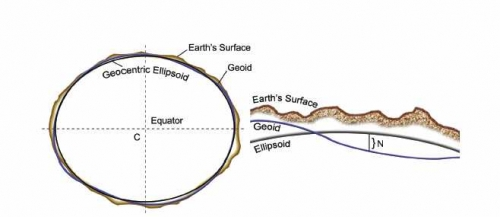
\includegraphics[width=0.8\textwidth]{images/geoid.jpg}
  \caption[Erde, Geoid und Referenzellipsoid]{Verhältnis zwischen der Erdoberfläche, dem Geoiden und einem Referenzellipsoiden. \cite{geodesy}}
  \label{fig:geoid}
\end{figure}

Die Wissenschaft der Erdvermessung - auch Geodäsie - beschäftigt sich mit dem Studium von Grösse und Form der Erde, des Erdgravitationsfeldes und den Veränderungen des eben genannten. Zu den Grundlagen der Geodäsie gehört die Unterscheidung zwischen der physikalischen Erde, dem Geoid und dem Referenzellipsoid. Die physikalische Erde ist die Erde an sich. Der Geoid hat die Form, welche eine von Ozeanen bedeckte Erde, nur unter Einfluss von Gravitation und Rotation annehmen würde. Der Referenzellipsoid ist eine einfache, mathematische Form welche dem Geoid so gut als möglich entspricht. \cite{geodesy}

\subsection{Georeferenzierung}
Die Fähigkeit geografische Positionen genau zu beschreiben ist essentiell für sowohl Karten als auch geografische Informationssysteme. Diesen Prozess nennt man Georeferenzierung.

Eine geografische Position mithilfe von Längen- und Breitengraden auf dem Referenzellipsoiden zu beschreiben ist eine Art der Georeferenzierung. Weitere Möglichkeiten wäre zum Beispiel die Verwendung von planaren oder kartesischen Koordinatensystemen. Im Umgang mit GPS werden ausschliesslich Längen- und Breitengrade verwendet, weshalb die weiteren Möglichkeiten im Rahmen dieser Arbeit nicht weiter erläutert werden.

Die Längen- und Breitengrade sind Winkelmessungen wischen dem Zentrum des entsprechenden Ellipsoiden und einem Punkt auf der Oberfläche. Breitengrade (in Englisch latitude) messen dabei den Winkel in Nord-Süd Richtung, Längengrade (in Englisch longitude) den Ost-West Winkel. \cite{georef}

\begin{figure}[h]
  \centering
  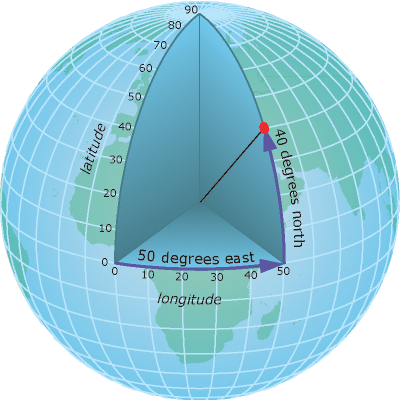
\includegraphics[width=0.5\textwidth]{images/longlat.png}
  \caption[Längen- und Breitengrade]{Lesen von Längen- und Breitengraden \cite{georef}}
  \label{fig:longlat}
\end{figure}

\subsection{World Geodetic System 1984}
Das World Geodetic System 1984 ist das geodätische Referenzsystem welches für GPS Positionsangaben verwendet wird. Als Koordinatenursprung dieses Systems dient das Massenzentrum der Erde. 

Dieses System besteht aus:
\begin{itemize}
	\item einem Referenzellipsoid für Ortsangaben nach geographischer Länge und Breite
	\item einem Geoid
	\item einem Satz dreidimensionaler Koordinaten der zwölf über die Erde verteilten Fundamentalstationen für die Verankerung der zuvor genannten Modelle in der Erdkruste \cite{wsg84}
\end{itemize}

\subsection{Global Positioning System}
GPS Besteht aus drei Segmenten, dem Raumsegment, dem Kontrollsegment und dem Nutzersegment. Das Raumsegment ist so konzipiert, dass es aus 24 bestehen soll, die die Erde in einer Höhe von rund 20200km alle 12 Stunden umrunden. Des weiteren ist das Raumsegment so angelegt, dass immer mindestens 4 Sateliten über einem Mindestelevationswinkel von 15$^\circ$ sichtbar sind. Jeder GPS-Satellit hat mehrere hochgenaue Atomuhren an Bord. Die Uhren arbeiten mit einer Grundfrequenz von 10.23 Mhz, die gebraucht wird, um das von den Satelliten gesendete Signal zu generieren. \cite{leicagps}

\begin{figure}[h]
  \centering
  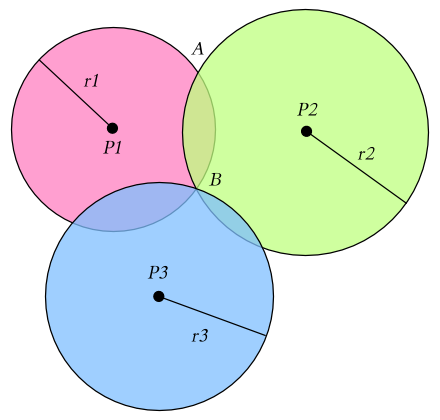
\includegraphics[width=0.6\textwidth]{images/trilateration.png}
  \caption[Trilateration]{Trilateration \cite{trilateration}}
  \label{fig:trilateration}
\end{figure}

Das Kontrollsegment besteht aus einer Hauptkontrollstation, der sogenannten Master Control Station (MCS), 5 Monitorstationen und 4 Telemetriestationen (Bodenantennen) verteilt über 5 Orte, die in etwa auf dem Äquator liegen.\cite{leicagps}

Das Kontrollsegment verfolgt die GPS-Satelliten, aktualisiert ihre Umlaufposition und kalibriert sowie synchronisiert ihre Uhren.\cite{leicagps}

Eine weitere wichtige Funktion ist, die Umlaufbahn eines jeden Satelliten zu bestimmen und seinen Weg für die nächsten 24 Stunden vorherzusagen. Diese Information wird jedem Satelliten eingespeist, um anschliessend von ihm gesendet zu werden. Damit ist der GPS-Empfänger in der Lage zu wissen, wo jeder einzelne Satellit erwartungsgemäss zu finden sein wird.\cite{leicagps}

Das Nutzersegment umfasst all diejenigen, die einen GPS-Empfänger einsetzen, um das GPS-Signal zu empfangen und so ihre Position und / oder Zeit zu bestimmen. Typische Anwendungen innerhalb des Nutzersegments sind die Navigation auf Land für Wanderer, die Bestimmung von Fahrzeugpositionen oder die Vermessung, die Navigation auf See, Navigation in der Luftfahrt, Maschinensteuerung usw. \cite{leicagps}

Die Positionsbestimmung per GPS basiert auf dem Prinzip der Trilateration. Der GPS Empfänger kennt die Position der GPS Sateliten und kann die Distanz zu jedem der Sateliten bestimmen. Wenn die Entfernung zu einem Sateliten bekannt ist, kann die eigene Position nur auf einer Kugelschale mit der Distanz als Radius und dem Sateliten als Mittelpunkt liegen. Durch den Schnitt dreier imaginärer Kugelschalen kann die Empfängerposition bestimmt werden. In der Abbildung \ref{fig:trilateration} ist dieses Prinzip - der einfachheitshalber in 2D - ersichtlich. \cite{leicagps}

\subsection{Distanzberechnung zwischen GPS Koordinaten}
\label{subsec:basicscalcdistance}
Zur Berechnung der Distanz zwischen zwei GPS Koordinaten wurde in dieser Arbeit die Haversine Formel verwendet: \cite{haversine} 

Definitionen:\\
\begin{equation}
\begin{array}{lcl}
\varphi_1, \varphi_2 & = & \text{Breitengrade}\\
\lambda_1, \lambda_2 & = & \text{Längengrade}\\
\Delta\varphi & = & \text{Differenz zwischen den Breitengraden}\\
\Delta\lambda & = & \text{Differenz zwischen den Längengraden}\\
R & = & \text{Radius der Erde}\\
\end{array}
\end{equation}

Berechnung:\\
\begin{equation}
\begin{array}{lcl}
a & = &\sin^2(\frac{\Delta\varphi}{2})+\cos \varphi_1 \cdot \cos \varphi_2 \cdot \sin^2(\frac{\Delta\lambda}{2})\\
c & = & 2 \cdot atan2(\sqrt{a}, \sqrt{(1-a)})\\
d & = & R \cdot c
\end{array}
\end{equation}

Diese Formel verwendet anstelle des Ellipsoiden eine Sphäre was bei grossen Distanzen zu Fehlern führen kann. Bei den Distanzen zwischen Messpunkten von Velotouren oder Wanderungen ist dieser Fehler nicht signifikant. Die Vorteile dieser Formel liegen in der einfachen Implementierbarkeit und der guten Performanz dieser Implementationen. 

\subsection{Das GPX Datenformat}
Das GPX oder GPS Exchange Format ist ein XML Schema zur Darstellung von GPS Daten. Es kann verwendet werden um \flqq Waypoints\frqq, \flqq Tracks\frqq und \flqq Routes\frqq darzustellen. Eine Ansammlung von \flqq Waypoints\frqq kann verwendet werden um eine Menge von Punkten darzustellen die in keinem sequenziellen Zusammenhang zueinander stehen. \flqq Routes\frqq und \flqq Tracks\frqq beinhalten sequenziell angeordnete \flqq Waypoints\frqq. Der Unterschied zwischen den Beiden ist, dass bei einer \flqq Route\frqq nur Wegpunkte bei Richtungsänderungen abgebildet sind, den Rest muss sich das System daraus berechnen. Ein \flqq Track\frqq beinhaltet alle aufgezeichneten Punkte. Im Rahmen dieses Projektes werden \flqq Tracks\frqq aufgezeichnet. \cite{gpxwiki} \cite{gpx}

\begin{lstlisting}[language=XML, caption={GPX Beispielfile}]
<?xml version="1.0" ?>
<gpx creator="ch.zhaw.gpstracker" version="1.0" xmlns="http://www.topografix.com/GPX/1/0" xmlns:xsi="http://www.w3.org/2001/XMLSchema-instance" xsi:schemaLocation="http://www.topografix.com/GPX/1/0 http://www.topografix.com/GPX/1/0/gpx.xsd">
    <bounds maxlat="8.28439892" maxlon="8.28439892" minlat="8.28439892" minlon="8.28439892"/>
    <trk>
        <name><![CDATA[Baden-Oberrohrdorf]]></name>
        <trkseg>
            <trkpt lat="47.48865993" lon="8.22070903">
                <ele>379.0</ele>
                <time>2014-06-17T13:38:56Z</time>
                <sym>Dot</sym>
            </trkpt>
            <trkpt lat="47.48859126" lon="8.22059915">
                <ele>378.0</ele>
                <time>2014-06-17T13:39:04Z</time>
                <sym>Dot</sym>
            </trkpt>
            <trkpt lat="47.48381748" lon="8.28364061">
                <ele>410.0</ele>
                <time>2014-06-17T13:57:49Z</time>
                <sym>Dot</sym>
            </trkpt>
        </trkseg>
    </trk>
</gpx>
\end{lstlisting}
\clearpage
\section{Umsetzung}
Bei der Konzeptionierung und Entwicklung der Android App wurde Wert darauf gelegt, dass Programmlogik, Benutzeroberfläche, Exportfunktion und Datenbankanbindung soweit als möglich voneinander getrennt sind. Entsprechend sind diese Themen hier auch unabhängig voneinander beschrieben.

\subsection{Programmlogik / Backend}
\label{subsec:programmlogikbackend}
Das Backend unserer Android Applikation besteht aus den beiden Klassen Track und Waypoint. 

\begin{figure}[h]
  \centering
  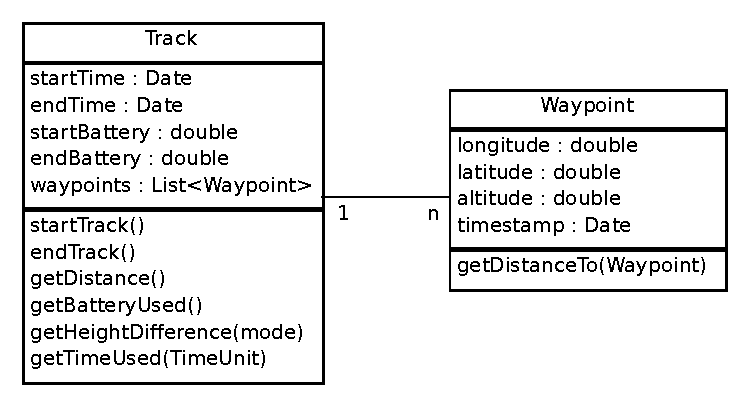
\includegraphics[width=0.8\textwidth]{images/classdiag_backend.pdf}
  \caption[Klassendiagramm Backend]{Klassendiagramm Backend}
  \label{fig:classdiag_backend}
\end{figure}

Im Klassendiagramm (Abbildung \ref{fig:classdiag_backend}) ist ersichtlich, dass ein Track primär aus einer Menge von Waypoints besteht. Zusätzlich werden Informationen zu Start- und Endzeit und Akkuzustand bei Start beziehungsweise Ende des Tracks mitgeführt. Die Waypoints bestehn aus den Koordinaten (Breiten- und Längengraden), der Höhe (Höhe über dem Geoiden) und einem Timestamp.

Der Track besitzt öffentliche Methoden zum Berechnen des Akkuverbrauchs, der Distanz, der Höhendifferenz und der Verbrauchten Zeit. Folgend wird kurz aufgezeigt wie die Funktionsweise dieser Methoden ist.

\begin{itemize}
\item \lstinline$getBatteryUsed()$ : $batteryUsed = startBattery-endBattery$ 
\item \lstinline$getDistance()$ : Siehe Kapitel \ref{subsec:distance}
\item \lstinline$getHeightDifference(mode)$ : Siehe Kapitel \ref{subsec:heightdifference}
\item \lstinline$getTimeUsed(TimeUnit)$ :
\begin{itemize}
	\item $timeUsedMs = endTime-startTime$
	\item $timeUsedS = \frac{endTime-startTime}{1000}$
	\item $timeUsedM = \frac{endTime-startTime}{1000*60}$
	\item $timeUsedH = \frac{endTime-startTime}{1000*60*60}$
	\item $timeUsedD = \frac{endTime-startTime}{1000*60*60*24}$
\end{itemize}
\end{itemize}

Weiter gibt es in der Klasse Track die beiden Methoden \lstinline$startTrack()$ und \lstinline$endTrack$, welche das Tracking an sich steuern. In der Methode \lstinline$startTrack$ (Listing \ref{lst:starttrack}) werden zuerst die beiden Einstellungen mithilfe des Android \lstinline$PreferenceManager$ ausgelesen. Als nächstes wird die StartZeit und der Batteriezustand beim Starten des Tracks festgehalten. Zum Schluss wird auf den \lstinline$LocationManager$ mithilfe des per Parameter übergebenen Contexts zugegriffen. Diesem \lstinline$LocationManager$ wird dann ein neuer \lstinline$LocationListener$ angehängt.

Beim Anhängen des \lstinline$LocationListener$s werden folgende Paramter mitgegeben: 
\begin{itemize}
	\item provider: Der Verwendete Provider für die Location Updates (in unserem Falle GPS)
	\item timeInterval: Das Zeitinterval. Wie oft soll der LocationListener angestossen werden?
	\item minDistance: Die minimale Distanz zwischen der aktuellen Location und der letzten. Wenn nach Ablauf des Zeitintervals diese Distanz nicht überschritten ist, wird der LocationListener nicht angestossen. \cite{locationmanager}
\end{itemize}

\begin{lstlisting}[caption={startTrack Methode}, label={lst:starttrack}]
private LocationListener = new LocationListener() {
	public void onLocationChanged(Location location) {
		// Called when a new location is found by the network location provider.
		trackLocation(location);
	}
}

public void startTrack(Context context) {
	//Read Settings
	SharedPreferences sharedPref = PreferenceManager.getDefaultSharedPreferences(context);
	long minDistance = Long.parseLong(sharedPref.getString("min_dist_between_tp", "10"));
	long timeInterval = Long.parseLong(sharedPref.getString("max_time_between_tp", "10000"));
	
	//set meta infos
	startTimestamp = new Date();
	startBatteryPercentage = getBatteryStatus(context);

	// Acquire a reference to the system Location Manager
	LocationManager locationManager = (LocationManager) context.getSystemService(Context.LOCATION_SERVICE);

	// Register the listener with the Location Manager to receive location updates
	locationManager.requestLocationUpdates(LocationManager.GPS_PROVIDER, timeInterval, minDistance, locationListener);
}
\end{lstlisting}

Das auslesen des Batteriezustandes geschieht dabei in der privaten Methode \lstinline$getBatteryStatus$, welche im Kapitel \ref{subsec:battery} weiter erläutert ist.

Das Abschliessen eines Tracks ist in der Methode \lstinline$endTrack$ abgebildet. Als erstes wird der verwendete \lstinline$LocationListener$ vom \lstinline$LocationManager$ getrennt. Danach wird geprüft, ob Wegpunkte aufgezeichnet wurden, falls nicht wird \lstinline$false$ zurückgegeben. Wenn Wegpunkte vorhanden sind, werden Zeit und Batteriezustand bei Ende des Tracks auf das Objekt geschrieben und das Objekt wird in der Datenbank abgelegt. Die Datenbankanbindung wird im Kapitel \ref{subsec:database} weiter erläutert.

\begin{lstlisting}[caption={endTrack Methode}, label={lst:endtrack}]
public boolean endTrack(Context context) {
	LocationManager locationManager = (LocationManager) context.getSystemService(Context.LOCATION_SERVICE);
	locationManager.removeUpdates(locationListener);

	if (waypoints == null || waypoints.size() == 0) {
		return false;
	} else {
		endTimestamp = new Date();
		endBatteryPercentage = getBatteryStatus(context);

		TracksDataSource tds = new TracksDataSource(context);
		tds.open();
		tds.createTrack(this);
		tds.close();

		return true;
	}
}
\end{lstlisting}

\subsection{Datenbankanbindung}
\label{subsec:database}
Zum persistieren der Backend Objekte (\lstinline$Waypoint$ und \lstinline$Track$) wurde das - bei Android Applikationen übliche - Content Provider Pattern \cite{contentprovider} zur Ansteuerung einer SQLite Datenbank verwendet. 

\begin{figure}[h]
  \centering
  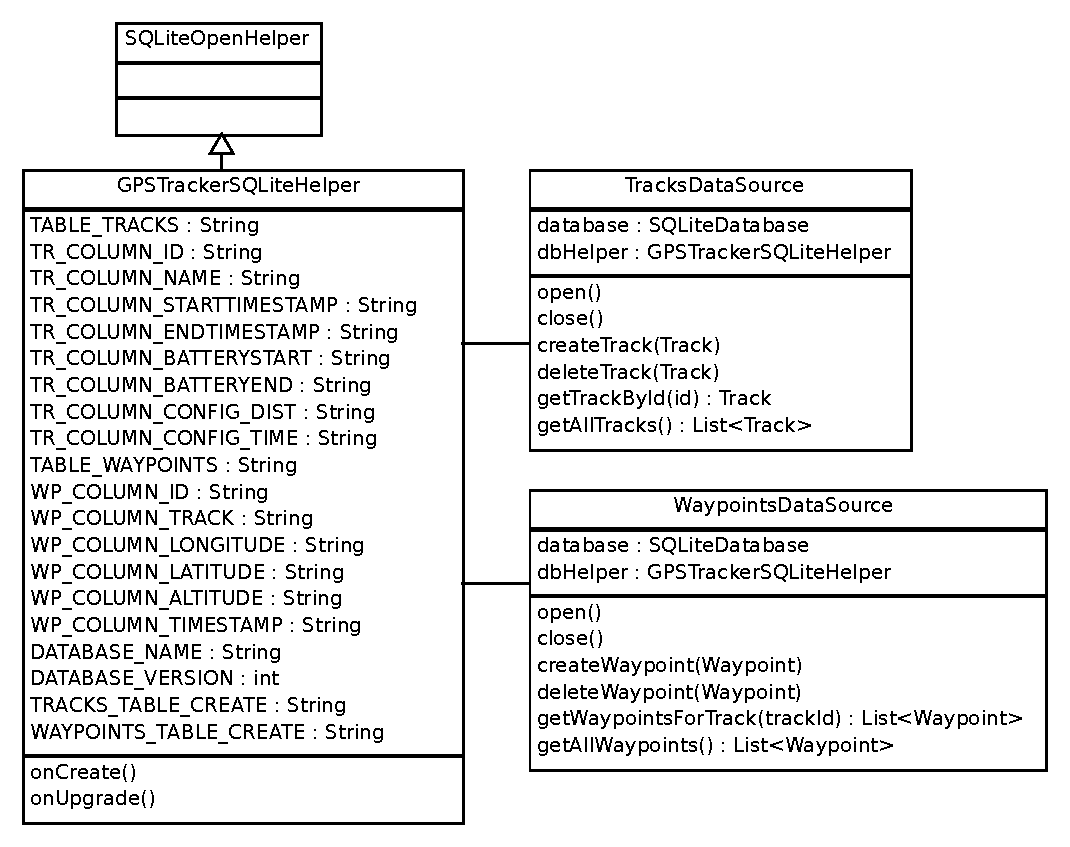
\includegraphics[width=0.6\textwidth]{images/classdiag_database.pdf}
  \caption[Klassendiagramm Datenbankanbindung]{Klassendiagramm Datenbankanbindung}
  \label{fig:classdiag_database}
\end{figure}

Zum Initialisieren der Datenbank und als Speicherort für die verwendeten Spalten- und Tabellennamen wurde der \lstinline$GPSTrackerSQLiteHelper$ verwendet. Dieser Helper ist von der Klasse SQLiteOpenHelper abgeleitet und überschreibt deren Methoden \lstinline$onCreate()$ und \lstinline$onUpdate()$. Die erstere wird aufgerufen, wenn die Datenbank noch nicht auf dem Device vorhanden ist. Die letztere wird aufgerufen, wenn die \lstinline$DATABASE_VERISON$ höher ist als diejenige, die beim erstellen der Datenbank auf dem Device aktuell war.

\lstinline$TracksDataSource$ und \lstinline$WaypointsDataSource$ bieten neben den $open()$ und $close()$ Methoden, welche eine Verbindung zur Datenbank herstellen beziehungsweise die Verbindung wieder trennen, ein Subset der üblichen CRUD \cite{crud} Methoden an, um die notwendigen Datenbankzugriffe auf eine möglichst einfache Art und Weise zu Verwalten. Im Listing \ref{lst:savetrackexample} ist an einem Beispiel ersichtlich, wie die \lstinline$TracksDataSource$ Klasse verwendet wird.

\begin{lstlisting}[caption={Beispiel: Track speichern}, label={lst:savetrackexample}]
TracksDataSource tds = new TracksDataSource(context);
tds.open(); //Connect database
tds.createTrack(track); //save track as new record 
tds.close(); //Close database connection
\end{lstlisting}

\subsection{Berechnung der Distanz}
\label{subsec:distance}
Die Distanz zwischen zwei Wegpunkten wird gemäss der Haversine Formel (Siehe Kapitel \ref{subsec:basicscalcdistance}) berechnet. Implementiert ist dies als Methode \lstinline$getDistanceTo(Waypoint)$ welche die Distanz zwischen dem aufrufenden und dem per Parameter übergebenen Waypoint, wie in Listing \ref{lst:distancecalc} ersichtlich, berechnet. Die Distanz eines ganzen Tracks entspricht der Summe der Distanzen zwischen allen Wegpunkten und ist in der Methode \lstinline$getDistance()$ der Track Klasse implementiert.

\begin{lstlisting}[caption={Distanzberechnung}, label={lst:distancecalc}]
private final static int R = 6371;
public double getDistanceTo(Waypoint other){
	double loThis = Math.toRadians(this.getLongitude());
	double laThis = Math.toRadians(this.getLatitude());
	double loOther = Math.toRadians(other.getLongitude());
	double laOther = Math.toRadians(other.getLatitude());
	
	double deltaLa = laThis-laOther;
	double deltaLo = loThis-loOther;
	
	double a = Math.pow(Math.sin(deltaLa/2), 2) + Math.cos(laThis) * Math.cos(laOther) * Math.pow(Math.sin(deltaLo/2), 2);
	double c = 2 * Math.atan2(Math.sqrt(a), Math.sqrt(1-a));
	return = R * c;
}
\end{lstlisting}

\subsection{Berechnung der Höhendifferenz}
\label{subsec:heightdifference}
Die Berechnung der Höhendifferenz (Listing \ref{lst:heightDifference}) hat drei Verschiedene Modi. Der Grund dafür lässt sich am besten an einem Beispiel erklären: Wenn man mit dem Velo von Göschenen (Rund 1100 m.ü.M.) auf den Gotthard Pass (rund 2100 m.ü.M) und danach weiter nach Airolo (rund 1175 m.ü.M) fährt, ist die Gesamthöhendifferenz 75 Meter. Abhängig von der körperlichen Verfassung wird der Velofahrer die 1000m, die er hoch gestrampelt ist, trotzdem in den Beinen spüren und entsprechend möchte er eine solche Angabe auch in einem GPS Tracker angezeigt bekommen. Basierend auf dieser Anforderung wurden die folgenden drei Modi entwickelt:

\begin{itemize}
\item positive: Die Summe aller Teilstrecken-Höhendifferenzen die positiv sind. (Im Gotthard Beispiel wären dies die ca. 1000m Bergauf)
\item negative: Die Summe aller Teilstrecken-Höhendifferenzen die negativ sind. (Im Gotthard Beispiel wären dies die ca. 925m Bergab)
\item total: Die Summe aller Teilstrecken-Höhendifferenzen. (Im Gotthard Beispiel ca. 75m)
\end{itemize}

\begin{lstlisting}[caption={Berechnung der Höhendifferenz}, label={lst:heightDifference}]
public double getHeightDifference(String mode) {
	if (waypoints.size() == 0 || waypoints.size() == 1) { //Cannot calculate height difference without waypoints
		return 0;
	} else {
		double sum = 0;
		for (int i = 1; i <= waypoints.size() - 1; i++) {
			double div = waypoints.get(i).getAltitude() - waypoints.get(i - 1).getAltitude();
			switch (mode) {
				case "positive": //only count positive height difference
					sum += div > 0 ? div : 0; break;
				case "negative": //only count negative height difference
					sum += div < 0 ? (-1) * div : 0; break;
				case "total": //count everything
					sum += div; break;
			}
		}
		return sum;
	}
}
\end{lstlisting}


\subsection{Akkumessung}
\label{subsec:battery}
Das auslesen der Batteriezustandes ist in der Privaten Methode \lstinline$getBatteryStatus$ des Tracks mithilfe des \lstinline$Intent.ACTION_BATTERY_CHANGED$ implementiert. Die Mtehode liest den Zustand der Batterie aus und gibt diesen als \lstinline$double$ zwischen 0 und 1 zurück. Mithilfe des Intents können sowohl \lstinline$level$ (Integer zwischen 0 und einem gerätespezifischen Maximum) als auch \lstinline$scale$ (Integer der dem gerätespezifischen Maximum entspricht) ausgelesen werden. Eine geräteunabhängige Angabe zwischen 0 und 1 berechnet sich daraus wie folgt: $batteryStatus=\frac{level}{scale}$ \cite{batterystatus}
\begin{lstlisting}[caption={Auslesen des Batterystatus}, label={lst:batterystatus}]
private double getBatteryStatus(Context context) {
	IntentFilter ifilter = new IntentFilter(Intent.ACTION_BATTERY_CHANGED);
	Intent batteryStatus = context.registerReceiver(null, ifilter);
	int level = batteryStatus.getIntExtra(BatteryManager.EXTRA_LEVEL, -1);
	int scale = batteryStatus.getIntExtra(BatteryManager.EXTRA_SCALE, -1);
	double batteryPct = level / (double) scale;
	return batteryPct;
}
\end{lstlisting}

\subsection{Android Frontend}
Das Android Frontend ist sehr einfach gestrickt. Es besteht aus drei Activities: Der \lstinline$SettingsActivity$, welche verwendet wird um die GPS-Tracking Parameter zu konfigurieren, der \lstinline$TrackListActivity$ welche die Track Liste anzeigt und der \lstinline$TrackDetailActivity$ - die Detailansicht für die einzelnen Tracks. Sowohl die TrackList als auch das TrackDetail Sheet wurden in Fragments (\lstinline$TrackListFragment$ und \lstinline$TrackDetailFragment$) so implementiert, dass auf einem Tablet nur eine Activity benötigt würde. Auf der linken Seite würde auf einem Tablet die Liste angezeigt und im Zentrum die jeweiligen Detail-Sheets.

\begin{figure}[h]
  \centering
  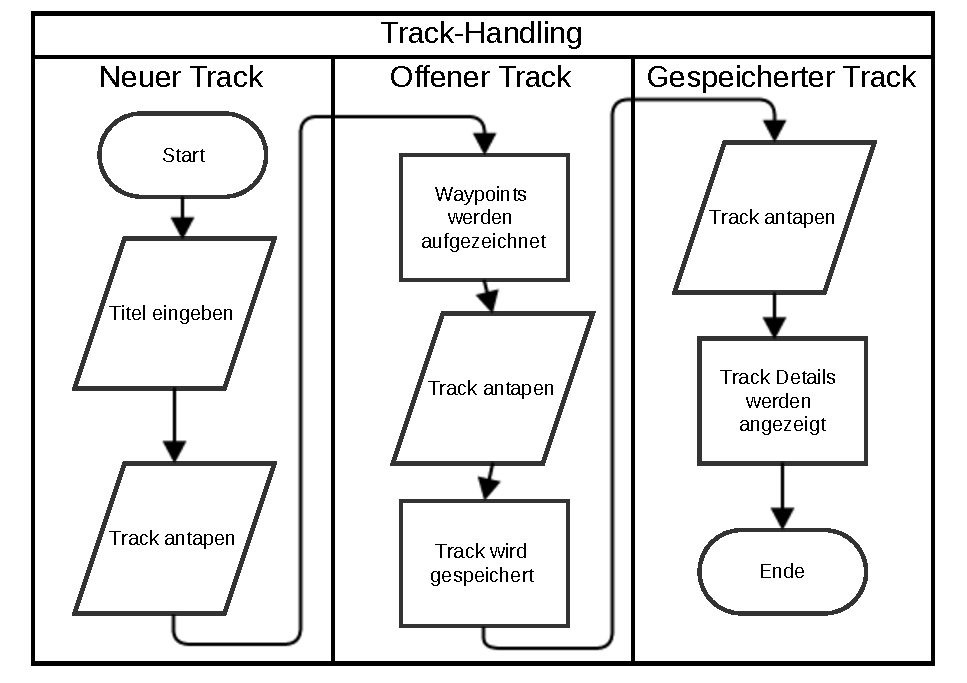
\includegraphics[width=0.8\textwidth]{images/trackworkflow.pdf}
  \caption[Track Lifecycle]{Track Lifecycle}
  \label{fig:tracklifecycle}
\end{figure}

Die Benutzerschnittstelle zum Erstellen von Tracks und zum Starten beziehungsweise Beenden des Trackings wurde so einfach wie möglich gehalten. In der Abbildung \ref{fig:tracklifecycle} ist in einem Flowchart der Track Lifecycle ersichtlich. Zum Erstellen eines Tracks, klickt der Benutzer aus der \lstinline$TrackList$ den Add Track Button. Nach dem Anklicken dieses Buttons wird der Benutzer nach einem Namen für den Track gefragt. Wenn er diesen eingibt und mit Ok bestätigt ist der Track als neuer Track in der Liste ersichtlich. Neue Tracks sind durch ein Play Symbol markiert. Wenn ein neuer Track angeklickt wird, beginnt der Trackingvorgang. Erneutes Anklicken beendet diesen und schreibt den Track in die Datenbank. Wenn gespeicherte Tracks angeklickt werden, öffnet sich das Detail-Sheet auf welchem verschiedene Informationen zum Track angezeigt werden.

\subsection{GPX Export}
\begin{figure}[h]
  \centering
  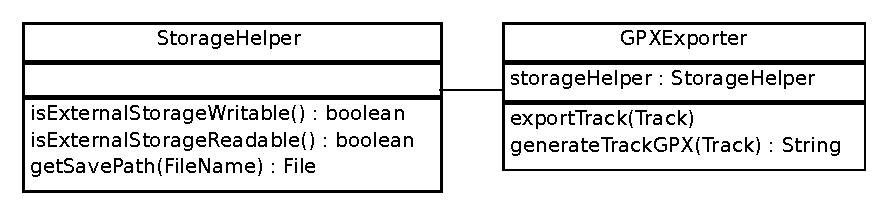
\includegraphics[width=0.6\textwidth]{images/classdiag_exporter.pdf}
  \caption[Klassendiagramm GPX Export]{Klassendiagramm GPX Export}
  \label{fig:gpxclassdiag}
\end{figure}

Das Exportieren von Tracks ins GPX Format wurde in der Klasse \lstinline$GPXExporter$ umgesetzt. Die Klasse bietet die zwei Methoden \lstinline$generateTrackGPX$ und \lstinline$exportTrack$ an. Die erstere nimmt einen Track entgegen und generiert daraus einen GPX XML String nach Spezifikation \cite{gpx}. Die letztere nimmt einen Track entgegen, findet mithilfe der entsrechenden Helper Klasse einen geeigneten Dateinamen auf Basis des Tracknamens, generiert das GPX XML mithilfe der \lstinline$generateTrackGPX$ Methode und schreibt dieses in das entsprechende File. Die Files werden im \lstinline$getExternalFilesDir(Environment.DIRECTORY_DOCUMENTS)$ \cite{savingfiles} abgelegt. Auf dieses Verzeichnis kann von einem PC aus zugegriffen werden. Wo genau es liegt, hängt vom verwendeten Gerät ab. 

Um Sicherzustellen, dass das externe Directory beschreibbar ist, wurde im Helper die Methode \lstinline$isExternalStorageWritable()$ implementiert, welche wie folgt prüft, ob das Verzeichnis beschreibbar ist:

\begin{lstlisting}[caption={Die isExternalStorageWritable Methode}, label={lst:isexternalstoragewriteable}]
public boolean isExternalStorageWritable() {
    String state = Environment.getExternalStorageState();
    if (Environment.MEDIA_MOUNTED.equals(state)) {
        return true;
    }
    return false;
}
\end{lstlisting}
\clearpage
\section{Analyse}
\subsection{Genauigkeit und Verwendbarkeit der Daten}
\label{subsec:analyseprecision}
Die GPS Daten die mit dem verwendeten Gerät (Google Nexus 5) aufgezeichnet wurden, sind - wie für GPS üblich \cite{gpsprecision} - bis auf wenige Meter genau. Die Genauigkeit hängt dabei vor Allem von der Umgebung ab. In Tunneln oder in engen Häuserschluchten ist der Empfang schlechter als auf einem offenen Feld oder im Wald. 

\begin{figure}[h]
  \centering
  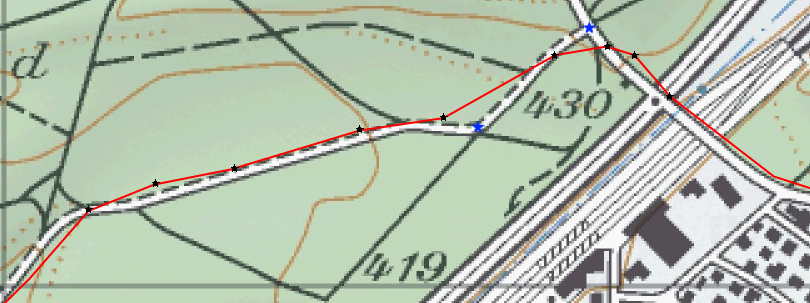
\includegraphics[width=\textwidth]{images/map_issues_10s.png}
  \caption[Genauigkeitsprobleme - zu wenige Datenpunkte]{Genauigkeitsprobleme - zu wenige Datenpunkte}
  \label{fig:precisionissues10s}
\end{figure}

Probleme durch diese Ungenauigkeit sind vor allem aufgetreten, wenn zu wenig Datenpunkte erfasst wurden. In der Abbildung \ref{fig:precisionissues10s} ist dies gut ersichtlich. Die Sternchen stehen für GPS Datenpunkte. Das erste Sternchen von Rechts liegt ziemlich gut auf der Strasse. Das Zweite ist aufgrund der GPS Ungenauigkeiten und äusseren Einflüssen um einige Meter daneben. Das Dritte ist wieder korrekt auf der Strasse. Zwischen dem Dritten und Vierten bin ich von der Strasse auf einen Waldweg abgebogen. Der vierte Datenpunkt liegt schön auf dem Waldweg, wird der Punkt an dem ich wirklich abgebogen bin (blauer Stern) nicht erfasst. Das Selbe geschieht zwischen dem vierten und fünften Datenpunkt. Diese Probleme lassen sich durch häufigeres Aufzeichnen der Daten minimieren.

\begin{figure}[h]
  \centering
  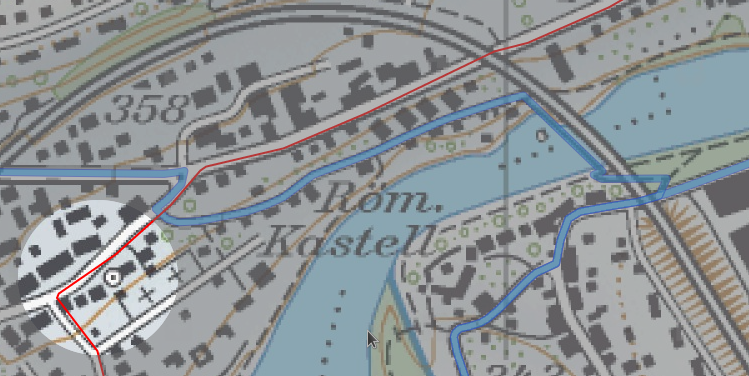
\includegraphics[width=0.9\textwidth]{images/map_issues_1s.png}
  \caption[GPS Ungenauigkeit]{GPS Ungenauigkeit}
  \label{fig:precisionissues1s}
\end{figure}

Bei einer genügenden Menge Datenpunkte wie in Abbildung \ref{fig:precisionissues1s} existieren immer noch Ungenauigkeiten. Die Route im markierten Bereich verläuft ein bis zwei Meter neben der Strasse. Jedoch wird hier im Gegensatz zur Abbildung \ref{fig:precisionissues10s} der Richtungswechsel problemlos korrekt eingezeichnet.

Man kann die Daten, sofern genügend Datenpunkte vorhanden sind, in der Form in welcher sie derzeit generiert werden durchaus verwenden um den Verlauf einer Fahrradtour festzuhalten. Die im Rahmen dieses Projektes aufgezeichneten Routen sind nicht befreit von Ungenauigkeiten, jedoch ist überall ersichtlich auf welcher Strasse ich gefahren bin. Um die vorhandenen Ungenauigkeiten zu minimieren, könnte man zum Beispiel einen  Map-Matching Filter anwenden wie er von Jason Daniel Martin et al. im Paper Dynamic GPS-position correction for mobile pedestrian navigation and orientation \cite{gpscorrection} vorgestellt wird. Um die Anzahl Datenpunkte zu verkleinern und um Ausreisser zu eliminieren könnten numerische Verfahren wie zum Beispiel der Ramer-Douglas-Peucker Algorithmus \cite{ramer}\cite{douglaspeucker} verwendet werden.

\subsection{Akkuverbrauch}
\label{subsec:analysebatteryusage}
Mit dem Java Android SDK ist es nicht möglich den Akkuverbrauch einer einzelnen Applikation zu messen. Was möglich ist, ist das Messen des aktuellen Akkustandes. In dem erstellen GPS Tracker wurde dies jeweils beim Start und nach Abschluss jedes Tracks getan. Die Auflösung dieser Messwerte sind auf 0.01 oder 1\% des Akkus genau.

Die Eingabeparameter des \lstinline$LocationManagers$ welche einen Einfluss auf den Akkuverbrauch des Trackers haben könnten, sind die im Kapitel \ref{subsec:programmlogikbackend} beschriebenen:
\begin{itemize}
	\item timeInterval
	\item minDistance
\end{itemize}

Wirklich relevant hierbei ist lediglich das \lstinline$timeInterval$. In diesen Abständen wird die GPS Location abgerufen. Um den Einfluss dieser Einstellung auf den Akkuverbrauch zu messen, wurden über rund drei Stunden Tracks mit verschiedenen Zeitintervallen aufgenommen:

\begin{figure}[h]
  \centering
  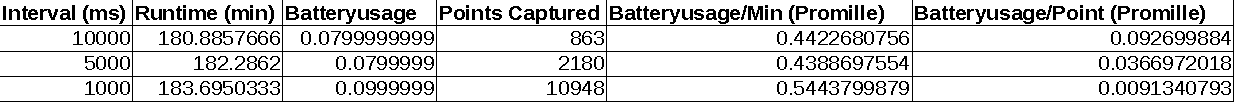
\includegraphics[width=\textwidth]{images/batteryusage.pdf}
  \caption[Statistik Akkuverbrauch]{Statistik Akkuverbrauch}
  \label{fig:batteryusage}
\end{figure}

In der Abbildung \ref{fig:batteryusage} sind die Resultate dieses Tests ersichtlich. Es hat sich kein markanter Unterschied des Akkuverbrauchs aufgrund dieser Konfigurationsparameter feststellen lässt. Dies deckt sich mit der Stackexchange Antwort vom Stackexchange User Jan:

\flqq The bigger thing is that you will be needing to keep the CPU powered on all the time. And, since you're using the PendingIntent flavor of requestLocationUpdates(), I am guessing that you plan on collecting data for a long time.\frqq

Er beschreibt, dass das Hauptproblem das ständige Arbeiten des Prozessors sei, welches zum Tracken der Location notwendig ist. Gemäss ihm sei es vor allem wichtig, dass man die \lstinline$LocationUpdates$ wieder ausschaltet wenn man sie nicht mehr braucht. Dies ist der Fall in dem hier hergestellten GPS Tracker.
\clearpage
\section{Fazit}
Trotz anfäglicher Schwierigkeiten und dem hohen Einarbeitungsaufwand in die Android Entwicklung, ist es gelungen einen Funktionsfähigen GPS Tracker zu entwickeln. Der Export ins GPX Format stellte keine Probleme dar. Die Optimierung des Akkuverbrauchs, welche zu Beginn im Fokus lag, war, wie im Kapitel \ref{subsec:analysebatteryusage} beschrieben, nicht erfolgreich. Jedoch hält sich der Akkuverbrauch in Grenzen, so dass auch Routen vom mehreren Stunden kein Problem darstellen dürften.

Um den GPS Tracker produktiv oder kommerziell nutzen zu können, müssten einige kleine Anpassungen vorgenommen werden. Zum Beispiel müssten Datenbankzugriffe und die Exportfunktion in separate Threads ausgelagert werden, so dass sie das Frontend nicht mehr blockieren. Weiter könnten die gewonnen Daten, zum Beispiel mit den im Kapitel \ref{subsec:analyseprecision} beschriebenen Techniken, verfeinert und optmiert werden.

Die Probleme mit der Androidentwicklung widerspiegeln sich auch im Vergleich zwischen der Soll- und der Ist-Planung des Projektes (Kapitel \ref{subsec:planung}). Ich musste deshalb vor allem Einschnitte in der Zeit zum Sammeln von Testdaten (dem Velofahren) in kauf nehmen. Auch die Dokumentation der Implementation wurde aus diesem Grund nach hinten verschoben, was sich unter anderem bei der Abgabe der ersten Rohfassung vom 04.06.2014 gezeigt hat.

\clearpage

%%%
%%% end main document
%%%
%%%%%%%%%%%%%%%%%%%%%%%%%%%%%%%%%%%%%%%%%%%%%%%%%%%%%%%%%%%%%%%%%%%%%%%%%%%%%%%%

 \appendix  %% include it, if something (bibliography, index, ...) follows below
\begin{appendix}
%\input{content/99_anhang/anhang.tex}
\printglossary[title=Glossar]
%%% start a new page and display the list of figures
% \newpage
 \listoffigures

%%% start a new page and display the list of tables
% \newpage
 \listoftables

\lstlistoflistings


%%%%%%%%%%%%%%%%%%%%%%%%%%%%%%%%%%%%%%%%%%%%%%%%%%%%%%%%%%%%%%%%%%%%%%%%%%%%%%%%
%%%
%%% bibliography
%%%
%%% available styles: abbrv, acm, alpha, apalike, ieeetr, plain, siam, unsrt
%%%
 \bibliographystyle{plain}

%%% name of the bibliography file
 \bibliography{projekt.bib}

\end{appendix}
\end{document}
%%% }}}
%%% END OF FILE
%%%%%%%%%%%%%%%%%%%%%%%%%%%%%%%%%%%%%%%%%%%%%%%%%%%%%%%%%%%%%%%%%%%%%%%%%%%%%%%%
%% Local Variables:
%% mode: outline-minor
%% OPToutline-regexp: "%% .*"
%% OPTeval: (hide-body)
%% emerge-set-combine-versions-template: "%a\n%b\n"
%% End:
%% vim:foldmethod=marker
